\documentclass[a4paper]{article}

%% Language and font encodings
\usepackage[english]{babel}
\usepackage[utf8x]{inputenc}
\usepackage[T1]{fontenc}

%% Sets page size and margins
\usepackage[a4paper,top=3cm,bottom=2cm,left=3cm,right=3cm,marginparwidth=1.75cm]{geometry}

%% Useful packages
\usepackage{amsmath}
\usepackage{graphicx}
\usepackage[colorinlistoftodos]{todonotes}
\usepackage[colorlinks=true, allcolors=blue]{hyperref}
\usepackage{enumitem}
\usepackage{eso-pic} 
\usepackage{float} %Så figurer kan placeres et præcist sted

\title{Astrofysik} %skal rettes til chapter
\author{Sofie Bruun}

\begin{document}
\maketitle

\section{Kosmologi}
Kosmologi er læren om universets skabelse, udvikling og endeligt. Når vi snakker om universets størrelse, er det normalt det synlige univers, vi mener. Dette er den del af universet, hvor lys har nået hen til os, så vi kan observere det. Længere ude er informationen ikke nået frem til os endnu, så vi ved ikke hvor stort hele universet er. 

Det passer med \textbf{det kosmologiske princip}. Ifølge dette er universets love og konstanter ens overalt og massen er ligevægt fordelt (set fra en stor nok skala). Det kan deles op i to postulater: Universet er homogent (ens overalt) og isotropt (ser ens ud, uanset hvilken retning man kigger i). Det kosmologiske princip behøver ikke gælde, men vi har ikke observeret noget der bryder med det. Så normalt antager vi, det gælder, da det er det simpleste - vi har ingen grund til at tro universets egenskaber pludselig ændrer sig et sted.

\subsection{Rødforskydning}
\subsubsection{Dopplerforskydning}
Du kender nok til, at hvis en ambulance kører forbi, så lyder sirenen højere når den nærmer sig, og lavere når den kører væk. Det kalder vi \textbf{Dopplerforskydning}. %Find gerne lydklip til undervisningen
Dette er fordi lydbølgerne skubbes sammen og strækkes, afhængigt af hvilken fart de udsendes med i forhold til lytteren. Hvis en ambulance kører mod dig, og du står stille, vil du høre bølgerne sammenpresset. Men hvis du selv kører med samme hastighed foran ambulancen, så vil du høre dem på samme måde, som de bliver udsendt - altså på samme måde som hvis begge biler stod stille, da det er den relative hastighed, som er afgørende.

Det samme sker for lys. Hvis en ambulance kører væk vil både tonen blive dybere og lyset fra den en smule rødere. Bemærk dog at selvom fotoner og lydbølger har højere energi ved korte bølgelængder, så mister de ikke energi ved Dopplerforskydning - der er bare sket et skift i perspektivet man ser bølgerne fra. Fra bølgens eget synspunkt (hvis man følger den) har den samme bølgelængde og energi hele tiden.
\subsubsection{Kosmologisk rødforskydning}
Edwin Hubble opdagede i 1920'erne at galakser langt borte ser rødforskudte ud, men dette skyldes \underline{ikke} Dopplerforskydning fra galaksernes egenhastighed i forhold til os. Så ville vi have forventet, at lige så mange galakser var rødforskudte som blåforskudte, hvis de starter med en tilfældig hastighed. Og det gør de jo - for hvorfor skulle de have en særlig retning i forhold til os? Men Hubble opdagede, at galakserne oftere er rødforskudt, og jo længere væk de er, desto mere rødforskudte er de også. Det vil sige deres relative hastighed til os er større, desto længere væk de er. Derfor må rødforskydningen stamme fra at alting bevæger sig længere væk fra hinanden, som rosiner i en hævende bolle. Det er netop, hvad der sker - universets dej dvs. rumtiden hæver. Galakserne har lige ofte egenhastigheder der går mod os som fra os, men hastigheden, selve rummet udvider sig med, er vigtigere for galakser langt væk, altså når der er meget rum imellem, der kan udvide sig under lysets rejse mod os. 

Ved rødforskydning fra rummets udvidelse mister lyset rent faktisk energi i modsætning til almindelig Dopplerforskydning. Dette er selvfølgelig et brud på energibevarelse, men det er egentlig ikke et problem, da man ikke kan betragte universet som et lukket system, fordi det udvider sig. Energibevarelse gælder kun i lukkede systemer. \cite{Davis}

Måden man måler rødforskydningen er ved at at opsplitte lyset i dets forskellige bølgelængder dvs. tage spektrer af fjerne objekter og derefter genkende mønstre fra jordiske laboratorier. Niels Bohr opdagede at elektroner kun kan eksistere i bestemte baner om atomkernene, men ikke mellem disse. Hver bane har en bestemt energi, så elektronernes energi i atomer er kvantiseret, dvs. de findes kun i bestemte pakker. Når en elektron henfalder til en lavere tilstand, kommer den af med overskydende energi ved at udsende en foton. Og hvis en foton med passende energi rammer en elektron, kan fotonen blive absorberet, så elektron kommer op i en højere energitilstand. Hvis man har en stjerne, som udsender et bredt spektrum


Når vi kan genkende et mønster af absorptionsliner eller emitionslinjer, selvom det ligger forskudt ved andre bølgelængder end normalt, så kan vi finde rødforskydningen. Den er defineret som forskellen mellem observeret bølgelængde $\lambda_{obs}$ og laboratoriebølgelængde $\lambda_{lab}$ i forhold til laboratoriebølgelængden. Det er altså den relative forskydning i forhold til den oprindelige bølge.

\begin{align}
	z=\frac{\lambda_{obs}-\lambda_{lab}}{\lambda_{lab}}
\end{align}
Rødforskydningen $z$ er relateret til hastigheden $v$ således:
\begin{align}
	z+1=\sqrt{\frac{1+\frac{v}{c}}{1-\frac{v}{c}}}
\end{align}
For hastigheder meget langsommere end lysets hastighed i vakuum $c$, kan det forsimples til:
\begin{align}
	z\approx\frac{v}{c}
\end{align}

Hubble formulerede en lov, der beskriver den direkte proportionalitet mellem afstand og hastighed af galaksen:
\begin{align}
	v=H_0 D
\end{align}
Her er $v$ farten, $D$ er afstanden til galaksen, og $H_0$ er Hubbles konstant, som er den nuværende værdi af Hubble-parameteren (der ikke er konstant).
 
 


\subsection{Universets form}

Universet har samlet set en form. Vi har 3 tydelige rumdimensioner omkring os, og vi er vant til, at hvis man tegner to parallelle linjer, så vil de aldrig krydse, og en trekant har altid 180 grader. Men dette gælder kun i fladt rum! Forestil dig for eksempel en trekant tegnet på en globus; den vil faktisk have mere end 180 grader. På samme måde vil en trekant tegnet på en saddel have mindre end 180 grader, som på Figur \ref{shapes}. Når rummet er kugleformet, har det en positiv krumning, og når det er saddelformet har det en negativ krumning. I fladt rum er krumningen 0.

\begin{figure}[H]
\centering
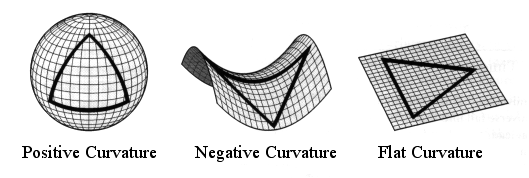
\includegraphics[width=0.7\textwidth]{universe_geometry.png}
\caption{Trekanter i forskellige rum har forskellige vinkelsummer. Billede fra http://abyss.uoregon.edu/~js/images/universe\_geometry.gif}
\label{shapes}
\end{figure}

Hvis et objekt er i frit fald, eller hvis man har en lysstråle, vil de bevæge sig langs en ret linje i rummet. Men hvis selve rummet krummer, så gør den "rette" linje det også. Derfor kan man ved at kigge på objekter langt væk se rummets krumning, da den vil vise sig i om ting ser forstørrede eller formindskede ud, og disse målinger viser at rummet er fladt med en præcision på 2 \%. %Kilde + illustration
Hvis rummet er positivt krumt og småt nok, ville det også betyde at lyset kunne nå hele vejen rundt, og vi ville se de samme objekter flere steder på himlen, hvilket heller ikke er observeret. Så det synlige univers er i hvert fald meget fladt - men måske har rummet en svag krumning, der bare ikke kan ses her. Selvom Danmark ser fladt ud, kan hele jordkloden jo godt være rund.

Hvis rummet er positivt krumt, er det endeligt, mens fladt eller negativt rum kan være uendeligt stort. Det er dog også muligt for rum både at være fx fladt og endeligt, men så bryder man det kosmologiske princip.

Vi kan sammenligne universets størrelse ved forskellige tidspunkter gennem en skalafaktor $a(t)$, hvor vi definerer den nuværende faktor til 1, $a(t_0)=1$, hvor $t_0$ er nu. Der gælder sammenhængen:
\begin{align}
	\frac{a(t_0)}{a(t)}=1+z
\end{align}
Så man kan let omregne rødforskydning til skalafaktoren, fra dengang lyset blev udsendt. Som beskrevet% i \ref{Hubble}
 tidligere er Hubblekonstanten ikke konstant, men er blot den nuværende Hubbleparameter. Hubbleparameteren er:
 \begin{align}
 H=\frac{v}{D}=\frac{\dot{a}}{a}
 \end{align}
 Hvis vi sætter det i anden, får vi \textbf{Friedmann-ligningen}:
\begin{align}
	H^2=\left(\frac{\dot{a}}{a}\right)^2=\frac{8\pi G \rho}{3}-\frac{\kappa c^2}{a^2}+\frac{\Lambda}{3}
\end{align}
Denne ligning er super interessant, da den viser os hvordan universet udvikler sig. Det er en andengradsligning med $a$ indeholdende konstanter som gravitationskonstanten $G$ og lysets fart $c$. $\kappa$ kan være 1, 0 og -1 og dette afgør krumningen, der som bekendt kan være positiv, 0 eller negativ. $\Lambda$ er den kosmologiske kontant. Uden denne ville rummet trække sig sammen, fordi massen krummer det, så Einstein introducerede $\Lambda$ for at holde universet statisk. Det har han senere kaldt sin største fejl, efter Hubble opdagede universet er dynamisk, men har man genintroduceret konstanten for at accelerere udvidelsen, da man opdagede mørk energi i 1998. 


\subsection{Universets komponenter} \label{bestanddele}
Universets skæbne afhænger af dets indhold. Det består af:
\begin{itemize}
	\item Stråling: Fotoner og neutrinoer (fordi de har ingen eller meget lav masse og høj hastighed)
	\item Stof: Almindeligt stof, antistof og mørkt stof har alle masse, så her kalder jeg dem samlet set "stof". Egenskaben masse afgør, hvor mange kræfter man skal bruge på at accelerere objekterne, men også hvor meget de krummer rummet omkring sig.
	\item Kosmologisk konstant: Den form for mørk energi, vi antager universet er fyldt med. Det får universets udvidelse til at accelerere, er ligeligt fordelt overalt og fortyndes ikke fra udvidelsen.
\end{itemize}

Disse komponenter påvirker universets form og udvikling forskelligt. Mængden af stof er nogenlunde konstant, men universet udvider sig i alle 3 rumdimensioner, så massedensiteten falder med:
\begin{align}
	\rho_m \propto R^{-3}
\end{align}
Stråling har ingen til næsten ingen hvilemasse, men ved høj fart får det en effektiv masse. Det er derfor lys ikke kan undslippe sorte hullers masse, selvom lyset ikke har en hvilemasse. Den effektive masse bøjer rummet omkring sig, så stråling får universet til at trække sig sammen, ligesom stof. Stråling har dog en ekstra egenskab, nemlig at det rødforskydes. Derfor fortyndes energien af stråling både med universets udvidelse og en ekstra faktor fra rødforskydningen:
\begin{align}
	\rho_R\propto R^{-4}
\end{align}

Mørk energi er ved man ikke særlig meget om, men man formoder det stammer fra energien i vakuum. Der er dog et ekstremt stort problem ved dette - vakuumenergien burde være $10^{120}$ gange større! Dette kan ses som et af mange usandsynlige tilfælde, der gør universet akkurat passer til liv kan opstå. Denne problemstilling er kendt som "the finetuning problem", og der er mange mulige løsninger på det, fx multiverser, virtuelle universer og brud på det kosmologiske princip gennem variende konstanter på tværs af sted. %\cite{TheAccUniverse} 
I den simple antagelse, at det består af "kosmologisk konstant", vil energien ikke fortyndes, så der hele tiden opstår mere mørk energi med udvidelsen og densiteten er:
\begin{align}
	\rho_\Lambda = konstant
\end{align}

Hvis universet er fladt kræver det en helt bestemt samlet densitet kaldet den kritiske densitet $\rho_c$. Lad os definere en densitetsparameter, som densitet i forhold til den kritiske densitet:
\begin{align}
	\Omega=\frac{\rho}{\rho_c}
\end{align}

%\subsection{References}
%\item Max Tegmark, \textit{Our Mathematical Universe: My Quest %for the Ultimate Nature of Reality}, 2014
%\item 
%\end{itemize}

\begin{thebibliography}{9}
\bibitem{Ryden}
Babara Ryden,
\textit{Introduction to Cosmology},
noget

\bibitem{Davis}
Tamara M. Davis,
\textit{Is the Universe Leaking Energy?},
Scientific American, 2010

\bibitem{TheAccUniverse}
P.W.C Davies
\textit{The Accidental Universe}
Cambridge University Press, Cambridge, 1982.

\end{thebibliography}
\end{document}